\documentclass[a4paper, 12pt]{article}
\usepackage[margin=1.25in, paperwidth=8.5in, paperheight=11in]{geometry}

\usepackage{graphicx}
\usepackage{float}
\usepackage{amsmath}
\usepackage{relsize}
\usepackage{bm}
\setlength\parindent{0pt}

\title{Mathematical \& Numeric Optimization}
\author{Matt Drury \& Cary Goltermann}

\begin{document}

\maketitle

\section*{Introduction}
    These notes will discuss the intuitions of numeric optimization via gradient descent. This intuition will be build via mathematical inspection of optimizable functions, examples of the coefficients for linear and logistic regression will be discussed at length. In addition, potential problems with the gradient descent algorithm will be pointed out along with some straightforward solutions; again, this is all in the pursuit of build intuition for the process.

\section*{Optimization}

\underline{Optimization} is the study of methods for finding the maximal of minimal value of a function.

\begin{figure}[H]
  \centering
    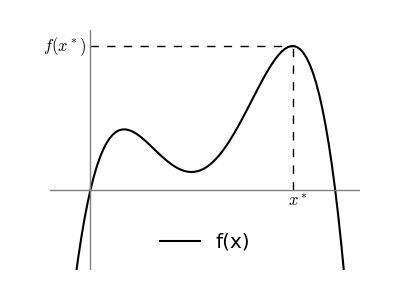
\includegraphics[scale=1]{images/one_var.png}
  \caption{One Variable Function} \label{fig:one}
\end{figure}

Figure \ref{fig:one} above plots a function of one variable, in it we see $x^*$, denoting the value of $x$ that yields the maximal value for $f(x)$, or the $argmax$ of $f$. If we were to optimize over this function the end goal would be to find the $x*$, the $argmax$ of $f$, thus providing us with knowledge about how to get the ``most'' out of $f$.

\vspace{1pc}

In figure \ref{fig:two} we can see the contours of a two-dimensional function plotted. \underline{Contour lines} have the property that the value of the function is the same at every point along the same line. These lines also go by the name \underline{level curves}. Again we can see the location in this space that yields the maximal value along this two-dimensional function, the $argmax$, labeled as $x^*$.

\begin{figure}[H]
  \centering
    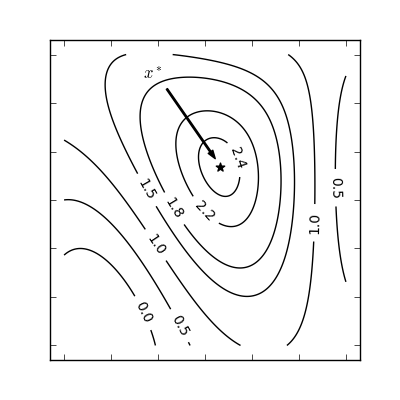
\includegraphics[scale=1]{images/two_var.png}
  \caption{Two Variable Function} \label{fig:two}
\end{figure}

\subsection*{Examples}
\begin{enumerate}
  \item \textbf{Linear Regression}

In linear regression we are trying to fit a line to our data, $\bm{X}$, in so doing finding optimal $\beta$'s that minimize the sum of squared errors.

    $$ \underset{\bm{\beta}}{\text{minimize}} \quad \mathlarger{\sum_{i=0}^n}
       \big(y_i - \sum_{j=0}^p \beta_j X_{ij} \big)^2 $$

This quantity sums over all the features in the data, $0-p$, and all the data points in the set, $0-n$. We can also express this with vector notation to reduce some of the indexing clutter.

    $$ \underset{\bm{\beta}}{\text{minimize}} \quad \Vert \bm{y} - \bm{X\beta} \Vert $$

  \item \textbf{Logistic Regression}

    In logistic regression we use the logistic, or sigmoid, $\sigma(x)$, link function to make probability predictions after taking the same linear combination we saw above in linear regression, $\bm{X\beta}$.

    $$ \sigma(x) = \frac{1}{1 + e^{-x}} $$

    We are interested in minimizing the total cross-entropy,

    $$ H(p, q) = - \sum_x p(x)\, log(q(x)), $$

    of these probabilities with the true labels from the set \{$0, 1$\} over all the data points.

    $$ \underset{\bm{\beta}}{\text{minimize}} \quad - \sum_{i=0}^n\,
       y_i\, log \big( \sigma(\bm{X}_i \bm{\beta})\big) +
       (1 - y_i)\, log \big( 1 - \sigma(\bm{X}_i \bm{\beta})\big) $$

    \qquad where
    $$ \bm{X}_i \bm{\beta} = \sum_{j=0}^p \bm{X}_{ij} \bm{\beta}_j$$.

\end{enumerate}

\section*{Constrained Optimization}

Sometimes optimization problems are \underline{constrained}. In these cases we are interested in the maximum/minimum value of $f$ but only in the cases that satisfy some constraints. An example constraint might be that we want the magnitude of the values in each dimension to be less than or equal to a certain threshold. We could represent such a constraint in two dimensions as such:

$$ x^2_1 + x^2_2 \leq M^2 $$

And so the optimization problem we would be facing could be written: maximize $f(x_1, x_2)$ subject to the constraint $ x^2_1 + x^2_2 \leq M^2 $.

\vspace{1pc}

This constraint can also be seen visually. In figure \ref{fig:two_const} below we see the same contour plot as above; however, now there is an added gray region with radius $M$ representing our constraint. The \underline{constraint region} in this example is circular due to the square terms in the above constraint.

\vspace{1pc}

We can see that the \underline{constrained maximum} of $f$, $x^*_{const}$, occurs at the first point that the constraint region touches a contour line of $f$.

\begin{figure}[H]
  \centering
    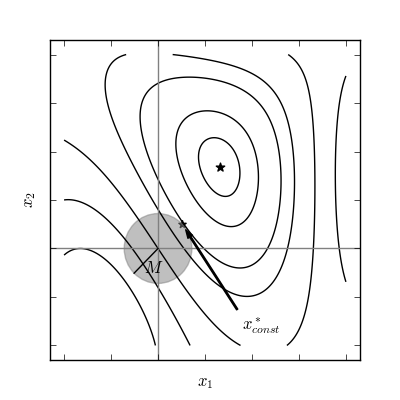
\includegraphics[scale=1]{images/two_var_constrained.png}
  \caption{Constrained Two Variable Function} \label{fig:two_const}
\end{figure}

\subsection*{Example}

\textbf{Regularized Linear Regression}

\vspace{0.5pc}

Sometimes, in linear regression, we want to control the magnitude of the betas that are learned by our model with the intuition that unrestrained betas can lead to overfitting. To constrain our betas all we simply add a term to our cost function summing up the squares of the betas and scaling that by some factor $\lambda$.

    $$ \underset{\bm{\beta}}{\text{minimize}} \quad \mathlarger{\sum_{i=0}^n}
       \big(y_i - \sum_{j=0}^p \beta_j X_{ij} \big)^2 + \lambda \sum_{j=0}^p \beta_j^2 $$

The magnitude of $\lambda$ is tuned as a hyperparameter with the intuition that larger values of $\lambda$ will make the effect of $\sum_j^n \beta_j^2$ larger, thus incentivizing smaller betas.

\vspace{1pc}

There is another, equivalent, way we can express this optimization problem; as a \underline{constrained} form of the linear regression cost function.

    $$ \underset{\bm{\beta}}{\text{minimize}} \quad \mathlarger{\sum_{i=0}^n}
       \big(y_i - \sum_{j=0}^p \beta_j X_{ij} \big)^2 $$

\qquad subject to the constraints:

    $$ \sum_{j=0}^p \beta_j^2 \leq M. $$

\subsection*{Legrange Multipliers}
This is representative of a general pattern:

\begin{quote}
  \textit{Every constrained optimization problem has an equivalent unconstrained optimization problem.}
\end{quote}

The process of moving from the constrained problem to the unconstrained problem is called \underline{Legrange Multipliers}.

\section*{The Gradient}

We want to develop methods for solving optimization problems, and all methods start with a common concept, the \underline{gradient}.

\subsection*{Definition}

Suppose that $f(\beta_0, \beta_1, \beta_2, ... , \beta_p)$ is a function of multiple arguments. The gradient of $f$ is the vector of the partial derivatives with respect to each of $f$'s inputs.

  $$ \nabla f(\beta_0, \beta_1, \beta_2, ... , \beta_p) = \bigg( \frac{\partial f}{\partial \beta_0}, \frac{\partial f}{\partial \beta_1}, \frac{\partial f}{\partial \beta_2}, ... , \frac{\partial f}{\partial \beta_p} \bigg) $$

Note, this vector depends on the point $(\beta_0, \beta_1, \beta_2, ... , \beta_p)$, this is why the gradient is sometimes referred to as a vector field.

\vspace{1pc}

Similarly to the derivative the gradient corresponds to the slope of hyperplane tangent to the function.

\subsection*{Properties}
\begin{itemize}
  \item The gradient at a point is perpendicular/orthogonal to the contour line that runs through that point, see figure \ref{fig:two_grad}.
  \item At a non-maximum/minimum, the gradient points in the direction that the function increases most quickly. 
  \item At a maximum/minimum (optima), the gradient is the \underline{zero} vector.
\end{itemize}

\begin{figure}[H]
  \centering
    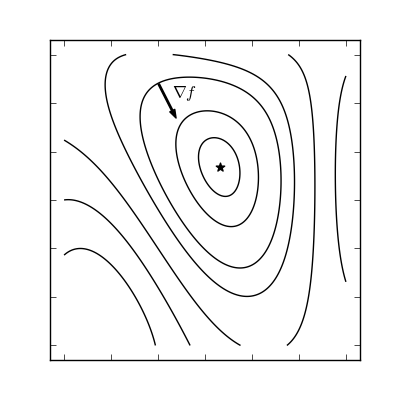
\includegraphics[scale=1]{images/two_var_gradient.png}
  \caption{Gradient for Two Variable Function} \label{fig:two_grad}
\end{figure}

\section*{Using the Gradient to Find Optima}

\subsection*{Solving Explicitly}

Very rarely, the following algorithm will result in a \underline{closed form} solution to finding an function's optima:

\begin{enumerate}
  \item Write down the function you want to optimize.
  \item Take all of the necessary partial derivatives to calculate the gradient of the function by hand. This sometimes fails.
  \item Set the gradient equal to the zero vector, and solve the resulting system of equations. This often fails.
\end{enumerate}

\subsection*{Example}

\begin{enumerate}
  \item Function: $f(\beta_1, \beta_2) = \beta_1^2 -2\beta_1 \beta_2 + 3\beta_2^2 + 4 \beta_1$
  \item The partial derivatives:
    \begin{align*}
      \frac{\partial f}{\partial \beta_1} & = 2\beta_1 - 2\beta_2 + 4 \\
      \frac{\partial f}{\partial \beta_2} & = -2\beta_1 + 6\beta_2
    \end{align*}
    $\Rightarrow$ Gradient: $\nabla f(\beta_1, \beta_2) = \big( 2\beta_1 - 2\beta_2 + 4, -2\beta_1 +6\beta_2 \big)$
  \item Set gradient equal to zero vector, yields system of equations:
    \begin{align*}
      2\beta_1 - 2\beta_2 & = 4 \\
      -2\beta_1 + 6\beta_2 & = 0
    \end{align*}
    This system can be solved with scipy and numpy:
    $scipy.linalg.solve(\left[
        \begin{smallmatrix}
            2 & -2 \\
            -2 & 6
        \end{smallmatrix}
        \right], \left[
        \begin{smallmatrix}
            -4 \\
            0
        \end{smallmatrix}
        \right])$.
      \vspace{0.5pc}
      The solution is at $(-3, -1)$, which is where the minimum of the function occurs.
\end{enumerate}

\subsection*{Example: Linear Regression}
If we apply the same procedure to the linear regression problem we get the result:

  $$ \hat{\beta} = scipy.linalg.solve(X^{\mathsmaller T}X, X^{\mathsmaller T} y), $$

\qquad which is often written as:

  $$ \hat{\beta} = (X^{\mathsmaller T}X)^{-1}X^{\mathsmaller T}y, $$

\qquad known as the normal equations.

\vspace{1pc}

Some people say that it's a miracle the ordinary least squares linear regression results in a closed from solution for the beta coefficients. As such it's important to know that linear regression exists as the exception, not the rule. In fact, the coefficients of logistic regression \textbf{can not} be solved for in this way.

\section*{Gradient Descent}

If explicit solutions often fail, how can we still optimize an arbitrary function? To answer this question we return to the defining property of the gradient at a point.

\begin{quote}
  \textit{The gradient points in the direction which the function increases most quickly.}
\end{quote}

With this definition in mind, consider the tactic of repeatedly walking in the direction of greatest increase, the gradient, or negative of the gradient for decrease.

\begin{figure}[H]
  \centering
    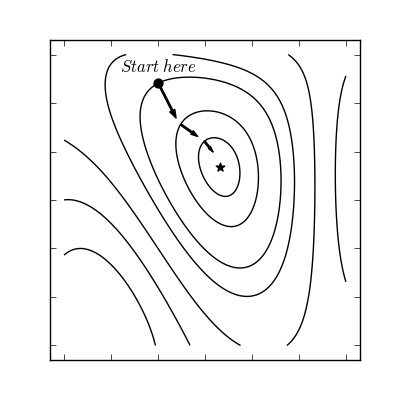
\includegraphics[scale=1]{images/two_var_gradient_descent.png}
  \caption{Gradient Descent for Two Variable Function} \label{fig:two_grad_desc}
\end{figure}

\subsection*{Algorithm}

\vspace{0.5pc}
There are two main parts to performing gradient descent.
\vspace{0.5pc}

\textbf{Pre-Algorithm}

\begin{itemize}
  \item Write down the function to optimize.
  \item Calculate the gradient analytically.
\end{itemize}

\textbf{Pseudocode}

\begin{itemize}
  \item Choose an initial point $x_0$.
  \item Until stopping criteria met:
    \begin{enumerate}
      \item Plug current point into gradient. $\nabla f(x_0)$.
      \item Move in the take a step along the gradient: \\
        \quad \textbullet \; $x_{i+1} \leftarrow x_i + \alpha \nabla f(x_0) \qquad$ \textbf{gradient ascent} \\
        \quad \textbullet \; $x_{i+1} \leftarrow x_i - \alpha \nabla f(x_0) \qquad$ \textbf{gradient descent}
      \item Repeat.
    \end{enumerate}
\end{itemize}

The learning rate, $\alpha$, corresponds to how far along the gradient vector you step each time. It is set to a positive number less than one, so as to guarantee we don't take too large a step and possibly ``overshoot'' our goal.

\subsection*{Stopping Criteria}
There are many ways that one can control how long you optimize for, the simplest is only iterating for a predetermined number of steps. There are, however, more sophisticated means of control.

\begin{enumerate}
  \item When $\Vert \nabla f \Vert < \epsilon$, where $\epsilon$, the \underline{convergence threshold}, is a small positive number. I.e. when the length of the gradient is small, almost the zero vector.
  \item When $\frac{\Vert f(x_{i+1}) - f(x_i) \Vert}{\Vert f(x_i) \Vert} < \epsilon$. I.e. when the percentage update is small.
\end{enumerate}

\section*{Trouble Shooting}

\subsection*{Local Optima}

When the function has multiple \underline{local} optima, gradient descent will converge to only one of them. In this case you may not end up anywhere near the \underline{global} optima. An illustration of this can be seen in figure \ref{fig:two_two_grad_desc}.

\vspace{1pc}

\textbf{Solutions}

\begin{itemize}
  \item Many common problems, e.g. linear/logistic regression, have exactly one local optima, so this issue does not arise. Functions like these are called \underline{globally convex}.
  \item Add an inertia term to your descent to "power through" getting stuck in a non-optimal local optima.
  \item In general, there is no silver bullet, you must add some randomization to your algorithm to try and get to better optima given different starting locations.
    \begin{itemize}
      \item Start at many random points. Choose the best optimal value from all that are found.
      \item Add some random noise to the gradient.
    \end{itemize}
\end{itemize}

\begin{figure}[H]
  \centering
    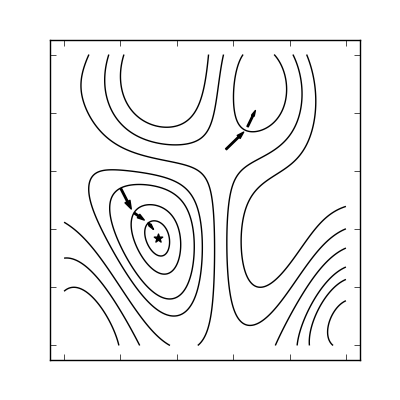
\includegraphics[scale=1]{images/two_var_gradient_descent_different_starts.png}
  \caption{Gradient Descent Starting from Different Initializations} \label{fig:two_two_grad_desc}
\end{figure}

\subsection*{Poorly Scaled Features}

In regression problems many times different features are measured on very different scales. e.g. measuring pounds a person weighs vs. height in feet. The other way we can see this problem is by realizing that whatever solution we come to should be invariant under constant transformations of our data. e.g. instead of measuring height in feet, converting everything to inches.

\vspace{1pc}

In this situation the level curves of the loss function become very long and thin, see figure \ref{fig:scaling_problems}. The ramification is that the gradient, which points in the direction of greatest assent in proportion to the rate of that change will predominantly point in the directions of the features that are on a larger scale.

\begin{figure}[H]
  \centering
    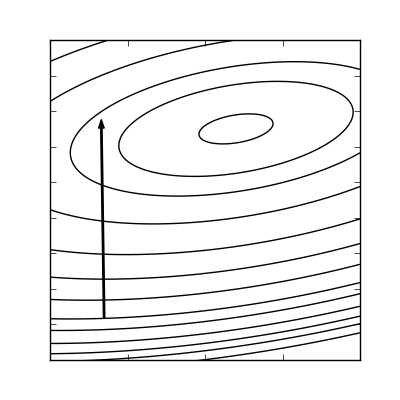
\includegraphics[scale=1]{images/scaling_problems.png}
  \caption{Poorly Scaled Features} \label{fig:scaling_problems}
\end{figure}

\vspace{1pc}

\textbf{Solution}: Scale the features!

\vspace{1pc}

Replace $\bm{X}_j$ with:
$$\frac{\bm{X}_j - mean(\bm{X}_j)}{std(\bm{X}_j)}.$$ 

This will make all of the features have mean zero and variance one. Graphically the level curves after standardizing are much more round.

\section*{Stochastic Gradient Descent}

The cost function of many important machine learning algorithms are \underline{sums} of a simpler function. These sums operate over all of the observations in our data set.

\vspace{1pc}

With this in mind, we can consider a computationally cheaper way to perform gradient descent by only considering what the gradient of our cost function is with respect to a single data point. This flavor of gradient descent is called \underline{stochastic gradient descent}, SGD, because we're adding some randomization to our descent path by only considering a single point for each update. The intuition here is that most of the time, though not always, the gradient of our loss function with respect to a single data point will generally point in the correct direction.

\vspace{1pc}

\textbf{Linear Regression}

\vspace{1pc}

Below we can see the equations for the linear regression loss with respect to an entire data set, $L(\bm{\beta}, \bm{X}, \bm{y})$, and with respect to a single data point, $l(\bm{\beta}, \bm{x}, y)$.

  \begin{align*}
    L(\bm{\beta}, \bm{X}, \bm{y}) &= \mathlarger{\sum_{i=1}^n}
                     \bigg(\bm{y}_i - \sum_{j=0}^p \bm{\beta}_j \bm{X}_{ij} \bigg)^2 \\
    l(\bm{\beta}, \bm{x}, y) &= \bigg(y - \sum_{j=0}^p \bm{\beta}_j \bm{x}_j \bigg)^2
  \end{align*}

\subsection*{Visualizing Stochastic Gradient Descent}

The effect of performing updates like this can be seen in figure \ref{fig:stochastic_path} below. We see that the path is not very direct, not necessarily moving in the ``best" direction, sometimes moving in the opposite way. But in aggregate it moves towards the optima quite well. 

\vspace{1pc}

This happens because, with respect to a single data point, the ``best" direction is not the same as the global ``best" at that location for the betas at that iteration.

\vspace{1pc}

In fact, we can see that the expectation of the gradient of the loss function with respect to a single data point is the average gradient.

  $$ E[\nabla l(\bm{\beta}, \bm{x}, y)] = \sum_{i=0}^n \frac{1}{n} \nabla l(\bm{\beta}, \bm{x}, y)
                                        = \nabla \frac{1}{n} \sum_{i=0}^n l(\bm{\beta}, \bm{x}, y) $$

This works because of the linearity of expectation and derivatives.

\subsection*{Why is Stochastic Gradient Descent Desirable}

Sometimes we don't have access to all of the data!

\begin{itemize}
  \item Huge datasets cannot fit into RAM.
  \item Our data is streaming to us, and we only have access to data temporarily.
  \item Our data is streaming to us, and we want to import our model in real time. This is called \underline{online learning}.
\end{itemize}

\begin{figure}[H]
  \centering
    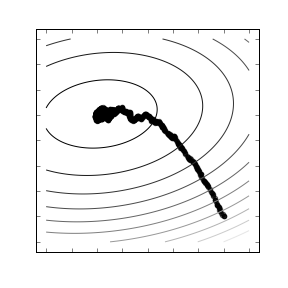
\includegraphics[scale=1]{images/stochastic.png}
  \caption{Stochastic Gradient Descent Path} \label{fig:stochastic_path}
\end{figure}

In addition, frequently we have to perform much fewer iterations, and therefor, calculations to converge to an optima. And getting computational gains is never a bad thing.

\subsection*{Comparing Gradient Descent with Stochastic}

\begin{itemize}
  \item \textbf{Gradient Descent}

    Updates, until convergence: $\bm{\beta}_{i+1} \leftarrow \bm{\beta}_i+ \alpha \; \frac{\partial}{\partial \bm{\beta}_i} L(\bm{\beta}_i, \bm{X})$. \\
    Here $\bm{X}$ is the entire training data set.

  \item \textbf{Stochastic Gradient Descent}

    Updates, until convergence: $\bm{\beta}_{i+1} \leftarrow \bm{\beta}_i+ \alpha \; \frac{\partial}{\partial \bm{\beta}_i} l(\bm{\beta}_i, \bm{x})$. \\
    Here $\bm{x}$ is a single observation from the training data set.
\end{itemize}

\subsection*{Deriving the Updates for Logistic Regression}

In logistic regression we are trying to find the best betas such that we minimize the cross-entropy of the predicted probabilities with their true labels. Or in math:

    $$ \underset{\bm{\beta}}{\text{minimize}} \quad - \sum_{i=0}^n\,
       y_i\, log \big( \sigma(\bm{X}_i \bm{\beta})\big) +
       (1 - y_i)\, log \big( 1 - \sigma(\bm{X}_i \bm{\beta})\big). $$

For the remainder of this example we will focus on the situation with a single data point, as we'd see in SGD, $\bm{x}$ to simplify notation. This makes our loss function, with respect to one data point:

    $$ \underset{\bm{\beta}}{\text{minimize}} \quad l(\bm{\beta}, \bm{x}, y) =
       - y \, log \big( \sigma(\bm{x} \bm{\beta})\big) -
       (1 - y) \, log \big( 1 - \sigma(\bm{x} \bm{\beta})\big). $$

Our gradient descent problem, then, is to find the derivative of the loss function, $l$, with respect to the betas, $\frac{\partial l}{\partial \bm{\beta}}$ in order to minimize the loss by iteratively updating our betas via step two in the pseudocode above.

\vspace{1pc}

To do this we'll use the chain rule:

  $$ \frac{\partial l}{\partial \bm{\beta}} = \frac{\partial l}{\partial \sigma(u)} \frac{\partial \sigma(u)}{\partial u(\bm{\beta})} \frac{\partial u(\bm{\beta})}{\partial \bm{\beta}}, $$

where $u(\bm{\beta}) = \bm{x \beta} \Rightarrow \frac{\partial u}{\partial \bm{\beta}} = \bm{x}$.

  $$ \frac{\partial l}{\partial \sigma} = -\frac{y}{\sigma} - \bigg(\frac{1-y}{1-\sigma} (-1)\bigg) = \frac{1-y}{1-\sigma} - \frac{y}{\sigma} $$

  \begin{align*}
    \sigma(u) &= \frac{1}{1 + e^{-u}} = \big(1 + e^{-u}\big)^{-1} \\
    &\Rightarrow \sigma + \sigma e^{-u} = 1 \\
    &\Rightarrow \frac{1 - \sigma}{\sigma} = e^{-u} \\
    &\Rightarrow e^{-u} = \frac{1}{\sigma} - 1 \\
    \Rightarrow \frac{\partial \sigma}{\partial u} &= -\big(1 + e^{-u}\big)^{-2}\big(-e^{-u}\big) = \big(1 + e^{-u}\big)^{-2}\big(e^{-u}\big)\\
    &= \sigma^2 (\frac{1}{\sigma} - 1) \\
    &= \sigma(1 - \sigma)
  \end{align*}

Putting all of this together.
  \begin{align*}
    \frac{\partial l}{\partial \bm{\beta}} &= \bigg(\frac{1-y}{1-\sigma} - \frac{y}{\sigma}\bigg) \big(\sigma(1 - \sigma)) \bm{x} \\
    &= \big((1 - y) \sigma - y (1 - \sigma)\big) \bm{x} \\
    &= \big(\sigma(\bm{x \beta}) - y\big) \bm{x}
  \end{align*}



\end{document}
